\documentclass[12pt]{article}
\usepackage{amsmath}
\usepackage{amsthm}
\usepackage{amsfonts}
\usepackage{amssymb}
\usepackage{enumitem}
\usepackage{tikz}
\usetikzlibrary{arrows.meta, calc, patterns, decorations.pathreplacing}
\usepackage[margin=.85in]{geometry}
\usepackage[colorlinks=true, allcolors=purple]{hyperref}
\pagestyle{empty}

\newcommand{\Rr}{\mathbb{R}}
\newcommand{\ihat}{\hat{\mathbf{i}}}
\newcommand{\jhat}{\hat{\mathbf{j}}}
\newcommand{\khat}{\hat{\mathbf{k}}}
\newcommand\abs[1]{\left|#1\right|}
\newcommand{\vv}[1]{\langle #1 \rangle}
\newcommand{\grad}{\nabla}
\newenvironment{solution}
  {\renewcommand\qedsymbol{$\blacksquare$}\begin{proof}[Solution]}
  {\end{proof}}

\begin{document}
\raggedright
\begin{center}
  {\large 2531 Selected Solutions}\\[2pt]
  \small A short, opinionated companion to \texttt{Calc3\_Outline.pdf}.
\end{center}

\noindent\textit{Each problem here earns its place by teaching an idea you carry forward, not a formula you forget. The spine is the gradient as one object read four ways, the recurring shape is the downward dome, and every surface gets its one dimensional companion curve first.}

\bigskip

%% ============================================================
\section{3D Coordinates and Vectors}
%% ============================================================

\paragraph{Problem.} \textit{Point $C$ lies on the segment from $A$ to $B$ with $|AC|=\tfrac12|CB|$. Writing $\vec a,\vec b,\vec c$ for the position vectors of $A,B,C$, show $\vec c=\tfrac23\vec a+\tfrac13\vec b$.}

\begin{solution}
A point on a segment is a weighted average of the ends, and the weights are the opposite pieces. Here $AC:CB=1:2$, so $C$ sits one third of the way from $A$ to $B$.
\[
  \vec c=\vec a+\tfrac13(\vec b-\vec a)=\tfrac23\vec a+\tfrac13\vec b.
\]
The end you stand nearer gets the bigger weight. This is the whole content of the midpoint formula and of every center of mass to come.
\end{solution}

\paragraph{Problem.} \textit{Let $\vec a=\langle1,0,2\rangle$, $\vec b=\langle-1,3,1\rangle$, $\vec c=\langle2,1,0\rangle$. Find the volume of the parallelepiped they span and the length of its main diagonal.}

\begin{solution}
The scalar triple product is the signed volume, base area times height in one stroke. $\vec b\times\vec c$ is the base normal, and dotting $\vec a$ onto it reads off the height.
\[
\vec b\times\vec c=\begin{vmatrix}\ihat&\jhat&\khat\\-1&3&1\\2&1&0\end{vmatrix}=\langle-1,2,-7\rangle,
\qquad \vec a\cdot(\vec b\times\vec c)=-1+0-14=-15.
\]
So $V=15$, the sign only recording orientation. The main diagonal runs to $\vec a+\vec b+\vec c=\langle2,4,3\rangle$, of length $\sqrt{4+16+9}=\sqrt{29}$.

\begin{center}
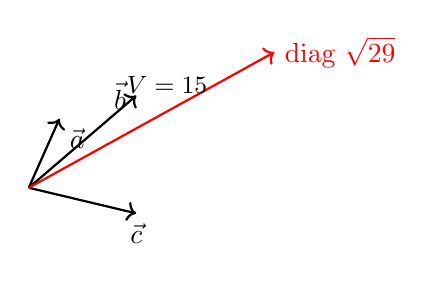
\begin{tikzpicture}[x={(0.6cm,-0.35cm)}, y={(0.9cm,0.2cm)}, z={(0cm,0.85cm)}, scale=0.65]
  \coordinate (O) at (0,0,0);
  \coordinate (A) at (1,0,2);
  \coordinate (B) at (-1,3,1);
  \coordinate (C) at (2,1,0);
  \coordinate (ABC) at (2,4,3);
  \draw[->,thick] (O)--(A) node[below right]{$\vec a$};
  \draw[->,thick] (O)--(B) node[left]{$\vec b$};
  \draw[->,thick] (O)--(C) node[below]{$\vec c$};
  \draw[->,red,thick] (O)--(ABC) node[right,red]{diag $\sqrt{29}$};
  \node at (1.5,2,2.5){\small $V=15$};
\end{tikzpicture}
\end{center}
\end{solution}

%% ============================================================
\section{Lines and Planes}
%% ============================================================

\paragraph{Problem.} \textit{Find the plane through $A(1,0,0)$, $B(0,2,0)$, $C(0,0,3)$.}

\begin{solution}
Two edges out of $A$ span the plane, and their cross product is the normal that turns the picture into one equation.
\[
  \overrightarrow{AB}=\langle-1,2,0\rangle,\quad \overrightarrow{AC}=\langle-1,0,3\rangle,\quad
  \vec n=\overrightarrow{AB}\times\overrightarrow{AC}=\langle6,3,2\rangle.
\]
Anchoring at $A$ gives $6(x-1)+3y+2z=0$, that is $6x+3y+2z=6$. The cross product earns its keep here, it is the direction the plane faces, not a number for its own sake.
\end{solution}

\paragraph{Problem.} \textit{Are the lines $\vec r_1=\langle1,2,0\rangle+t\langle1,-1,2\rangle$ and $\vec r_2=\langle2,1,3\rangle+s\langle2,1,-1\rangle$ parallel, intersecting, or skew?}

\begin{solution}
Two lines in space generically miss each other. Run the decision in order. The directions $\langle1,-1,2\rangle$ and $\langle2,1,-1\rangle$ are not multiples, so not parallel. To meet they must agree in all three coordinates at once. Matching $x$ and $y$,
\[
  1+t=2+2s,\qquad 2-t=1+s \;\Longrightarrow\; s=0,\ t=1.
\]
But then $z$ gives $2t=2$ on the first line and $3-s=3$ on the second. They disagree, so no parameters land on a common point. Not parallel and not meeting means skew, the two rails of a staircase.
\end{solution}

\paragraph{Problem.} \textit{Find the line where the planes $x+2y+z=4$ and $2x-y+z=3$ meet, and the angle between them.}

\begin{solution}
The common line lies in both planes, so it is perpendicular to both normals at once. That forces its direction to be the cross product.
\[
  \vec n_1=\langle1,2,1\rangle,\quad \vec n_2=\langle2,-1,1\rangle,\quad \vec n_1\times\vec n_2=\langle3,1,-5\rangle.
\]
Set $z=0$ and solve $x+2y=4$, $2x-y=3$ to get the point $(2,1,0)$, so $x=2+3t,\ y=1+t,\ z=-5t$. The angle between the planes is the angle between the normals,
\[
  \cos\theta=\frac{\vec n_1\cdot\vec n_2}{|\vec n_1||\vec n_2|}=\frac{2-2+1}{\sqrt6\,\sqrt6}=\frac16,
  \qquad \theta\approx 80.4^\circ.
\]
\end{solution}

\paragraph{Problem.} \textit{Does the line $x=1+t,\ y=2-t,\ z=3t$ cross the plane $2x+y-z=5$, run parallel to it, or lie inside it?}

\begin{solution}
The fast test is the line direction against the normal, but the cleanest route is to feed the line in and watch the parameter.
\[
  2(1+t)+(2-t)-3t=5 \;\Longrightarrow\; 4-2t=5 \;\Longrightarrow\; t=-\tfrac12.
\]
A single solution for $t$ means one clean hit, at $\bigl(\tfrac12,\tfrac52,-\tfrac32\bigr)$. Had the $t$ terms cancelled to a false statement the line would be parallel and outside, and to a true statement it would lie in the plane.
\end{solution}

%% ============================================================
\section{Quadric Surfaces}
%% ============================================================

\paragraph{Problem.} \textit{Sketch the ellipsoid $\dfrac{x^2}{4}+y^2+\dfrac{z^2}{9}=1$.}

\begin{solution}
Read a quadric by slicing it. Set one variable to a constant and see what curve falls out. Every coordinate plane here cuts an ellipse, with semi axes $2,1,3$ along $x,y,z$.

\begin{center}
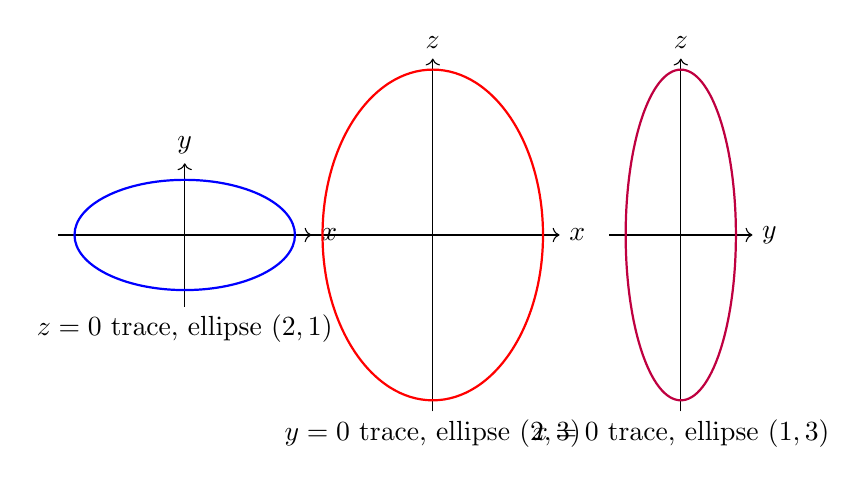
\begin{tikzpicture}[scale=0.7]
  \begin{scope}[xshift=-4.5cm]
    \draw[->](-2.3,0)--(2.3,0) node[right]{$x$};
    \draw[->](0,-1.3)--(0,1.3) node[above]{$y$};
    \draw[blue,thick] (0,0) ellipse (2 and 1);
    \node at (0,-1.7) {$z=0$ trace, ellipse $(2,1)$};
  \end{scope}
  \begin{scope}
    \draw[->](-2.3,0)--(2.3,0) node[right]{$x$};
    \draw[->](0,-3.2)--(0,3.2) node[above]{$z$};
    \draw[red,thick] (0,0) ellipse (2 and 3);
    \node at (0,-3.6) {$y=0$ trace, ellipse $(2,3)$};
  \end{scope}
  \begin{scope}[xshift=4.5cm]
    \draw[->](-1.3,0)--(1.3,0) node[right]{$y$};
    \draw[->](0,-3.2)--(0,3.2) node[above]{$z$};
    \draw[purple,thick] (0,0) ellipse (1 and 3);
    \node at (0,-3.6) {$x=0$ trace, ellipse $(1,3)$};
  \end{scope}
\end{tikzpicture}
\end{center}
\end{solution}

\paragraph{Problem.} \textit{Identify and sketch $z=y^2-x^2$, the saddle, by assembling it from slices.}

\begin{solution}
Build it from its companion curves. Walk along $y=0$ and you ride the downward parabola $z=-x^2$. Walk along $x=0$ and you ride the upward parabola $z=y^2$. One way down, the other up, so the origin is neither a peak nor a pit. The traces are
\begin{itemize}\itemsep1pt
  \item at $z=k>0$, a hyperbola $y^2-x^2=k$ opening in $\pm y$,
  \item at $z=k<0$, a hyperbola opening in $\pm x$,
  \item at $y=k$, the downward parabola $z=k^2-x^2$,
  \item at $x=k$, the upward parabola $z=y^2-k^2$.
\end{itemize}
The zero height lines $y=\pm x$ split the high ground from the low. This is the shape the second derivative test calls a saddle.

\begin{center}
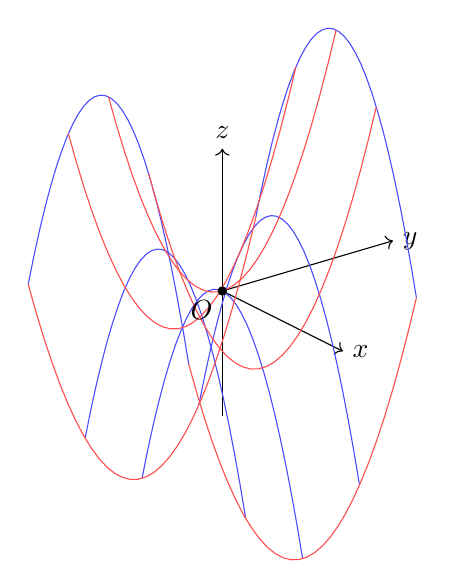
\begin{tikzpicture}[x={(0.6cm,-0.3cm)},y={(0.85cm,0.25cm)},z={(0cm,0.85cm)},scale=0.85]
  \draw[->](0,0,0)--(3,0,0)node[right]{$x$};
  \draw[->](0,0,0)--(0,3,0)node[right]{$y$};
  \draw[->](0,0,-2.2)--(0,0,2.5)node[above]{$z$};
  \foreach \yy in {-2,-1,0,1,2}{
    \draw[blue!70,thin,variable=\t,domain=-2:2,samples=30] plot (\t,\yy,{\yy*\yy-\t*\t});}
  \foreach \xx in {-2,-1,0,1,2}{
    \draw[red!70,thin,variable=\t,domain=-2:2,samples=30] plot (\xx,\t,{\t*\t-\xx*\xx});}
  \fill(0,0,0) circle(2pt) node[below left]{$O$};
\end{tikzpicture}
\end{center}
\end{solution}

\paragraph{Problem.} \textit{For $\dfrac{x^2}{9}-\dfrac{y^2}{4}+z^2=1$, find all coordinate plane traces and identify the surface.}

\begin{solution}
The traces are an ellipse one way and hyperbolas the other two,
\begin{itemize}\itemsep1pt
  \item at $z=0$, the hyperbola $\dfrac{x^2}{9}-\dfrac{y^2}{4}=1$ opening in $\pm x$,
  \item at $y=0$, the ellipse $\dfrac{x^2}{9}+z^2=1$ with semi axes $3$ and $1$,
  \item at $x=0$, the hyperbola $z^2-\dfrac{y^2}{4}=1$ opening in $\pm z$,
  \item at $y=k$, the ellipse $\dfrac{x^2}{9}+z^2=1+\dfrac{k^2}{4}$ growing with $|k|$.
\end{itemize}
Slices perpendicular to one axis stay ellipses while the other directions flare. That signature is a hyperboloid of one sheet, here with its waist along the $y$ axis.
\end{solution}

\paragraph{Problem.} \textit{Identify $x^2+y^2-z^2=1$ by its horizontal slices and its slice at $x=0$.}

\begin{solution}
At height $z=k$, $x^2+y^2=1+k^2$, a circle of radius $\sqrt{1+k^2}$. The waist at $z=0$ is the unit circle, and the circles grow as you leave it either way. The vertical slice $x=0$ is $y^2-z^2=1$, a hyperbola flaring open. Circles widening from a waist plus flaring sides is the cooling tower, a hyperboloid of one sheet with axis along $z$.
\end{solution}

%% ============================================================
\section{Space Curves and Vector Functions}
%% ============================================================

\paragraph{Problem.} \textit{Let $\vec r(t)=\langle\ln(t-1),\,\arctan t,\,\sqrt{4-t^2}\rangle$. Find the domain and sketch the $xy$ projection.}

\begin{solution}
The domain is the overlap of what each component allows. $\ln(t-1)$ needs $t>1$ and $\sqrt{4-t^2}$ needs $t\le2$, so the domain is $(1,2]$. As $t\to1^+$, $x\to-\infty$ while $y=\arctan t\to\pi/4$, and at $t=2$, $(x,y)=(0,\arctan 2)$. The curve enters from the far left along $y=\pi/4$ and ends at a point.
\end{solution}

\paragraph{Problem.} \textit{An electron has velocity $\vec v(t)=\langle -\sin t,\tfrac{1}{\sqrt2}\cos t,\tfrac{1}{\sqrt2}\cos t\rangle$ and starts at $\vec r(0)=\langle1,0,0\rangle$. Find $\vec r(t)$ and show it stays on a sphere.}

\begin{solution}
Integrate component by component, then pin the constant with the start.
\[
  \vec r(t)=\langle\cos t,\tfrac{\sin t}{\sqrt2},\tfrac{\sin t}{\sqrt2}\rangle,\qquad
  |\vec r|^2=\cos^2t+\tfrac{\sin^2t}{2}+\tfrac{\sin^2t}{2}=1.
\]
The length is locked at $1$ for all time, so the electron rides the unit sphere, which happens exactly because velocity stays perpendicular to position. The path is the great circle in the plane $y=z$.
\end{solution}

\paragraph{Problem.} \textit{The cylinder $x^2+y^2=1$ and the plane $z=x+y$ meet in a curve. Parametrize it and find the tangent line at $(1,0,1)$.}

\begin{solution}
Let the cylinder carry the parametrization and the plane set the height. On the cylinder $x=\cos t,\ y=\sin t$, and the plane forces $z=\cos t+\sin t$.
\[
  \vec r(t)=\langle\cos t,\sin t,\cos t+\sin t\rangle,\qquad \vec r\,'(t)=\langle-\sin t,\cos t,-\sin t+\cos t\rangle.
\]
The point $(1,0,1)$ is $t=0$, where $\vec r\,'(0)=\langle0,1,1\rangle$, so the tangent line is $\langle1,0,1\rangle+u\langle0,1,1\rangle$. The shadow on the floor is just the unit circle, which the plane tilts into a slanted ellipse in space.
\end{solution}

\paragraph{Problem.} \textit{Working from the definitions, find the unit tangent $\vec T$ and unit normal $\vec N$ for the circle $\vec r(t)=\langle a\cos t,a\sin t\rangle$ and the helix $\vec r(t)=\langle\cos t,\sin t,t\rangle$. Which way does $\vec N$ point?}

\begin{solution}
$\vec T$ is the direction of travel, $\vec N$ is where $\vec T$ is turning, always to the inside of the bend.

\medskip\noindent\textbf{Circle.} $\vec r\,'=\langle-a\sin t,a\cos t\rangle$ has length $a$, so $\vec T=\langle-\sin t,\cos t\rangle$ and $\vec N=\langle-\cos t,-\sin t\rangle$, pointing straight at the center. On a circle the inside of the turn is the middle, every time.

\medskip\noindent\textbf{Helix.} $\vec r\,'=\langle-\sin t,\cos t,1\rangle$ has length $\sqrt2$, so $\vec T=\tfrac{1}{\sqrt2}\langle-\sin t,\cos t,1\rangle$ and $\vec N=\langle-\cos t,-\sin t,0\rangle$. The normal is horizontal, aimed at the central axis, even as the curve climbs. The climb lives entirely in $\vec T$.
\end{solution}

\paragraph{Problem.} \textit{A ball is launched from $(0,2)$ at $20$ m/s, aimed $60^\circ$ above horizontal, under gravity $\vec a=\langle0,-10\rangle$. Split the acceleration into tangential and normal parts at launch and at the top.}

\begin{solution}
Gravity is one fixed downward vector, but the curve feels it two ways. The part along $\vec T$ changes the speed, the part along $\vec N$ bends the path.
\[
  \vec v(t)=\langle10,\,10\sqrt3-10t\rangle,\qquad a_T=\frac{\vec a\cdot\vec v}{|\vec v|},\qquad a_N=\frac{|\vec a\times\vec v|}{|\vec v|}=\frac{100}{|\vec v|}.
\]

\medskip\noindent\textbf{At launch} $\vec v=\langle10,10\sqrt3\rangle$, $|\vec v|=20$, so $a_T=-5\sqrt3\approx-8.7$ (slowing as it climbs) and $a_N=5$ (gravity also curving the path).

\medskip\noindent\textbf{At the top} the vertical speed is zero, $\vec v=\langle10,0\rangle$, $|\vec v|=10$, so $a_T=0$ (speed momentarily steady) and $a_N=10$. At the apex every bit of the pull goes into bending the arc.
\end{solution}

\paragraph{Problem.} \textit{Curvature of $y=x^2$ at the origin, then the ellipse $\dfrac{x^2}{4}+y^2=1$ at $(2,0)$ and $(0,1)$.}

\begin{solution}
Curvature is how hard a curve bends, and its reciprocal is the radius of the circle that fits snugly there. For $y=x^2$,
\[
  \kappa=\frac{|y''|}{(1+(y')^2)^{3/2}},\qquad \text{at }x=0,\ \kappa=\frac{2}{1}=2,
\]
so the kissing circle at the vertex has radius $\tfrac12$. For the ellipse $\vec r(t)=\langle2\cos t,\sin t\rangle$, the plane curvature is $\kappa=\dfrac{2}{|\vec r\,'|^3}$ with $|\vec r\,'|^2=4\sin^2t+\cos^2t$.

\medskip\noindent\textbf{At $(2,0)$, $t=0$} $|\vec r\,'|=1$, so $\kappa=2$, radius $\tfrac12$, center $\bigl(\tfrac32,0\bigr)$. The pointy end bends hard.

\medskip\noindent\textbf{At $(0,1)$, $t=\pi/2$} $|\vec r\,'|=2$, so $\kappa=\tfrac14$, radius $4$, center $(0,-3)$. The flat top bends gently.

\begin{center}
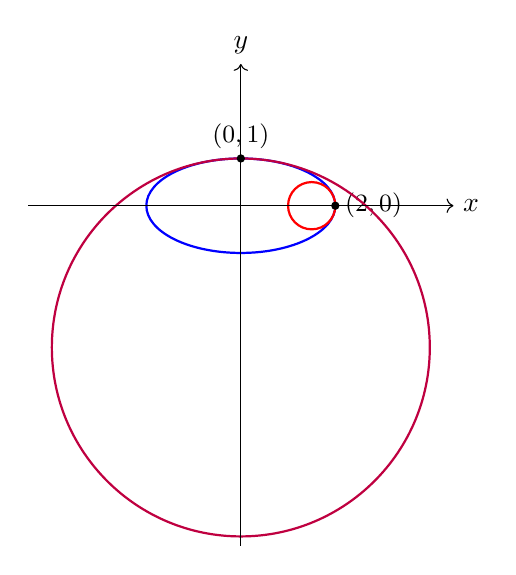
\begin{tikzpicture}[scale=0.6]
  \draw[blue,thick] (0,0) ellipse (2 and 1);
  \draw[red,thick] (1.5,0) circle(0.5);
  \fill(2,0) circle(2.5pt) node[right]{\small$(2,0)$};
  \draw[purple,thick] (0,-3) circle(4);
  \fill(0,1) circle(2.5pt) node[above]{\small$(0,1)$};
  \draw[->](-4.5,0)--(4.5,0)node[right]{$x$};
  \draw[->](0,-7.2)--(0,3)  node[above]{$y$};
\end{tikzpicture}
\end{center}
\end{solution}

\paragraph{Problem.} \textit{The curve $\vec R(t)=\langle t,t,1-2t^2\rangle$ is the dome $z=1-x^2-y^2$ cut along $y=x$, with $\vec R(\tfrac12)$ at $P=(\tfrac12,\tfrac12,\tfrac12)$. Find the curvature, the center of the osculating circle at $P$, and compare the direction from $P$ to that center with the dome's normal $\langle1,1,1\rangle$.}

\begin{solution}
\[
  \vec R\,'=\langle1,1,-4t\rangle,\qquad \vec R\,''=\langle0,0,-4\rangle.
\]
At $t=\tfrac12$, $\vec R\,'=\langle1,1,-2\rangle$ with $|\vec R\,'|=\sqrt6$, and the acceleration points straight down. Then
\[
  \vec R\,'\times\vec R\,''=\langle-4,4,0\rangle,\qquad
  \kappa=\frac{\sqrt{32}}{6\sqrt6}=\frac{2\sqrt3}{9}.
\]
So $\rho=1/\kappa=\tfrac{3\sqrt3}{2}$, and the center sits that far along the inward normal, down into the bowl, at $(-1,-1,-1)$. The direction from $P$ to the center is $\langle-\tfrac32,-\tfrac32,-\tfrac32\rangle$, exactly opposite the surface normal $\langle1,1,1\rangle$. Here the two genuinely agree as a line, the slice bending back toward the side the surface faces. Hold this against the later warning that the gradient need not point along the position vector. Agreement here is special, not the rule.
\end{solution}

%% ============================================================
\section{Functions of Multiple Variables}
%% ============================================================

\noindent\textit{The gradient is one object you read four ways. Dot it with a small displacement and you get the linear approximation. Dot it with a velocity and you get the chain rule. Dot it with a unit direction and you get the directional derivative. Set it to zero and you get the candidates for a max or min. The problems build each reading in one dimension first, then lift it. The recurring object is the downward dome $z=1-x^2-y^2$ at $P=(\tfrac12,\tfrac12,\tfrac12)$.}

\bigskip

\subsection*{The Gradient Four Ways}

\paragraph{Problem.} \textit{The dome $z=1-x^2-y^2$ at $P=(\tfrac12,\tfrac12,\tfrac12)$. (a) Find $\nabla f(P)$. (b) Use it to write the tangent plane and estimate $f(0.51,0.49)$. (c) Find the rate of climb at $P$ along $\vec u=\tfrac{1}{\sqrt2}\langle1,1\rangle$. (d) Where is the gradient zero, and what is there?}

\begin{solution}
$\nabla f=\langle-2x,-2y\rangle$, so $\nabla f(P)=\langle-1,-1\rangle$. One vector, read four ways.

\medskip\noindent\textbf{(b) Dot with a displacement to linearize.} The tangent plane is
\[
  L(x,y)=\tfrac12-(x-\tfrac12)-(y-\tfrac12)=\tfrac32-x-y.
\]
At $(0.51,0.49)$ the displacement is $\langle0.01,-0.01\rangle$ and $\nabla f(P)\cdot\langle0.01,-0.01\rangle=0$, so $L=\tfrac12$. The true value $f(0.51,0.49)=0.4998$ sits just under, because the dome bends below its tangent plane and the estimate runs high.

\medskip\noindent\textbf{(c) Dot with a unit direction for the directional derivative.}
\[
  D_{\vec u}f(P)=\nabla f(P)\cdot\vec u=\langle-1,-1\rangle\cdot\tfrac{1}{\sqrt2}\langle1,1\rangle=-\sqrt2.
\]
Walking the diagonal slice agrees. With $y=x$ parametrized by $\langle t,t\rangle$, $z=1-2t^2$ and $s=\sqrt2\,t$, so $\dfrac{dz}{ds}=\dfrac{-4t}{\sqrt2}$, which at $t=\tfrac12$ is $-\sqrt2$.

\medskip\noindent\textbf{(d) Set it to zero to optimize.} $\nabla f=\langle-2x,-2y\rangle=\vec0$ only at the origin, the peak $(0,0,1)$, where the dome has its maximum.
\end{solution}

\paragraph{Problem.} \textit{Build the tangent plane to the dome at $P$ from scratch, out of the two trace tangents, and confirm it is the linearization.}

\begin{solution}
Before the gradient hands you a formula, see where the plane comes from. Hold $y=\tfrac12$ and the dome becomes a curve in a vertical plane, whose tangent at $P$ has slope $f_x(P)=-1$, so $\vec a=\langle1,0,-1\rangle$ rides it. Hold $x=\tfrac12$ and the trace tangent is $\vec b=\langle0,1,-1\rangle$ with slope $f_y(P)=-1$. The plane through $P$ spanned by $\vec a,\vec b$ has normal
\[
  \vec a\times\vec b=\langle1,1,1\rangle,
\]
so $z=\tfrac32-x-y$, exactly the linearization. The two trace slopes are the two partials, and the plane is the unique flat thing matching both at once.
\end{solution}

\paragraph{Problem.} \textit{When does a tangent line over estimate and when does it under estimate? Build it in 1D, then lift to the dome.}

\begin{solution}
Take $f(x)=\sqrt x$ at $a=4$, so $f'(4)=\tfrac14$ and $L(4.1)=2.025$. The true value $\sqrt{4.1}=2.0249$ is a touch lower. The graph is concave down, so it bends beneath its tangent line and the line predicts too much. Flip the concavity and the line predicts too little. The sign of the error is the sign of the bend.

The same logic lifts. A tangent plane estimate is too high where the surface bends below the plane and too low where it bends above. The dome bends below everywhere, so its linearization always over estimates. A saddle bends below in one direction and above in another, so its plane neither over nor under estimates outright.
\end{solution}

\paragraph{Problem.} \textit{Find the tangent plane to the saddle $z=x^2+xy-y^2$ at $(1,1,1)$. Is the estimate from the plane always too high, always too low, or neither?}

\begin{solution}
$f_x=2x+y$ and $f_y=x-2y$, so at $(1,1)$ the gradient is $\langle3,-1\rangle$ and $z=3x-y-1$. Whether the estimate runs high or low is a question about shape. A saddle crosses through its tangent plane rather than staying on one side, so the estimate is too high along the falling direction and too low along the rising one. Neither verdict holds outright, the way it did for the dome.
\end{solution}

\subsection*{Domains, Level Sets, and Limits}

\paragraph{Problem.} \textit{Read partial derivatives off a contour map. Near $(2,1)$ the level curves of $f$ are the ellipses of $f=x^2/4+y^2$. Estimate $f_x(2,1)$ and $f_y(2,1)$, then check.}

\begin{solution}
A partial derivative is rise over run, and on a contour map the rise is the gap between labels and the run is how far you step. Stepping right from $(2,1)$ you cross contours, and the closer they pack the steeper the climb. The same step upward crosses them faster, since the ellipses crowd in the $y$ direction. Calculus confirms it, $f_x=\tfrac{x}{2}=1$ and $f_y=2y=2$, twice as steep up as right. The gradient $\langle1,2\rangle$ crosses every contour square and aims straight uphill.
\end{solution}

\paragraph{Problem.} \textit{Sketch the level curves of $f(x,y)=x^2+4y^2$ for $k=1,4,9$.}

\begin{solution}
$x^2+4y^2=k$ rewrites as $\dfrac{x^2}{k}+\dfrac{y^2}{k/4}=1$, an ellipse with semi axes $\sqrt k$ and $\sqrt k/2$. The contours are nested ellipses, squashed in $y$ because $f$ climbs faster there.
\end{solution}

\paragraph{Problem.} \textit{Sketch the domain of $f(x,y)=\ln(y-x^2)$.}

\begin{solution}
The log needs $y>x^2$, the open region above the parabola.
\end{solution}

\paragraph{Problem.} \textit{Evaluate $\displaystyle\lim_{(x,y)\to(0,0)}\frac{x^3+y^3}{x^2+y^2}$, and show $\displaystyle\lim_{(x,y)\to(0,0)}\frac{x^2-y^2}{x^2+y^2}$ does not exist.}

\begin{solution}
Polar coordinates expose the difference. The first becomes $r(\cos^3\theta+\sin^3\theta)$, and since $|\cos^3\theta+\sin^3\theta|\le2$ it is squeezed to $0$ as $r\to0$ for every angle. The limit is $0$. The second becomes $\cos2\theta$, with no $r$ at all, so the value is whatever ray you come in on, $1$ along $y=0$ and $-1$ along $x=0$. A limit that depends on direction does not exist.
\end{solution}

\subsection*{Chain Rule}

\paragraph{Problem.} \textit{Let $z=x^2y$, $x=r\cos\theta$, $y=r\sin\theta$. Find $\partial z/\partial\theta$ by the chain rule.}

\begin{solution}
The chain rule is the gradient dotted with the velocity of the moving inputs.
\[
  \frac{\partial z}{\partial\theta}=2xy(-r\sin\theta)+x^2(r\cos\theta)=r^3\cos\theta(\cos^2\theta-2\sin^2\theta).
\]
\end{solution}

\paragraph{Problem.} \textit{Reparametrize the dome by $x=s\cos t,\ y=s\sin t$. Find $\partial z/\partial s$ and $\partial z/\partial t$, and explain why $\partial z/\partial t=0$.}

\begin{solution}
In polar the dome is $z=1-s^2$, depending on $s$ alone, so $\partial z/\partial s=-2s$ and $\partial z/\partial t=0$. Spinning $t$ moves you around a circle of fixed radius, a level curve where the height never changes, so $\partial z/\partial t=0$ is the radial symmetry stated in one equation. At $(s,t)=(\tfrac{1}{\sqrt2},\tfrac{\pi}{4})$ you sit at $P$, and $\partial z/\partial s=-\sqrt2$, the same steepest descent rate as the directional derivative.
\end{solution}

\paragraph{Problem.} \textit{The length, width, and height of a box change in time. At one instant $\ell=1,\ w=2,\ h=2$ m with $\ell'=w'=2$ and $h'=-3$ m/s. How fast is the volume changing?}

\begin{solution}
$V=\ell wh$ depends on three moving quantities, so its rate is the chain rule summed over three paths.
\[
  \frac{dV}{dt}=wh\,\ell'+\ell h\,w'+\ell w\,h'=(4)(2)+(2)(2)+(2)(-3)=8+4-6=6.
\]
Growing at $6$ cubic meters per second. Each term is a face area times how fast the opposite dimension moves, the volume that face sweeps. Two faces push out and one pulls in, and the pushers win.
\end{solution}

\paragraph{Problem.} \textit{Show $u=f(x-at)+g(x+at)$ satisfies the wave equation $u_{tt}=a^2u_{xx}$.}

\begin{solution}
A right mover plus a left mover. With $\xi=x-at$ and $\eta=x+at$, $u_{tt}=a^2f''(\xi)+a^2g''(\eta)$ and $u_{xx}=f''(\xi)+g''(\eta)$, so $u_{tt}=a^2u_{xx}$. Any shape you like, sent left and right at speed $a$, solves the wave equation.
\end{solution}

\subsection*{Tangent Planes, Directional Derivatives, and Gradients}

\paragraph{Problem.} \textit{Tangent plane to $x^2+2y^2+3z^2=21$ at $(2,2,1)$, and the linearization of $f(x,y)=\sqrt{20-x^2-7y^2}$ at $(2,1)$ to estimate $f(1.95,1.08)$.}

\begin{solution}
For a surface written as a level set, the gradient is the normal, no solving for $z$ needed. $\nabla F=\langle2x,4y,6z\rangle=\langle4,8,6\rangle$, so the plane is $2x+4y+3z=15$. For the explicit graph, $f_x=-2/3$ and $f_y=-7/3$ at $(2,1)$ with $f(2,1)=3$, so
\[
  L(x,y)=3-\tfrac23(x-2)-\tfrac73(y-1),\qquad f(1.95,1.08)\approx2.847.
\]
\end{solution}

\paragraph{Problem.} \textit{Find the tangent plane and the normal line to the sphere $x^2+y^2+z^2=9$ at $(1,2,2)$.}

\begin{solution}
The gradient of the defining function gives both, because it is the one direction perpendicular to the surface. $\nabla F=\langle2,4,4\rangle\parallel\langle1,2,2\rangle$, so the tangent plane is $x+2y+2z=9$ and the normal line is $\langle1,2,2\rangle+t\langle1,2,2\rangle$, the radius extended. On a sphere the outward normal is always radial, the gradient confirming the geometry.
\end{solution}

\paragraph{Problem.} \textit{Directional derivative of $f(x,y)=x^2y^3$ at $P(1,2)$ in the direction $\vec v=\ihat+\jhat$, and the steepest climb.}

\begin{solution}
With $\hat u=\tfrac{1}{\sqrt2}\langle1,1\rangle$ and $\nabla f(1,2)=\langle16,12\rangle$,
\[
  D_{\hat u}f=\frac{16+12}{\sqrt2}=14\sqrt2.
\]
Over all directions the largest value is $|\nabla f|=20$, reached along $\nabla f$, the steepest climb. Pointing across it gives zero, the level direction.
\end{solution}

\paragraph{Problem.} \textit{Show $\nabla f$ is perpendicular to the level curve through a point, and that it need not point toward the origin. Use $f(x,y)=x^2+3y^2$.}

\begin{solution}
Walk along a level curve and $f$ holds steady, so the directional derivative along it is zero. But $D_{\hat u}f=\nabla f\cdot\hat u$, which vanishes exactly when $\nabla f$ is perpendicular to the tangent direction. So the gradient crosses every level curve at a right angle and points the way $f$ grows fastest. For $f=x^2+3y^2$, whose level curves are ellipses squashed in $y$, $\nabla f=\langle2x,6y\rangle$. At $(1,1)$, $\nabla f=\langle2,6\rangle$, not a multiple of the position $\langle1,1\rangle$. It leans toward the $y$ axis where the surface climbs harder. Only on the axes does the gradient line up with the radius.
\end{solution}

\paragraph{Problem.} \textit{A solid has temperature $F(x,y,z)=x^2+2y^2+3z^2$. (a) Show $P(1,2,1)$ is on $F=12$. (b) Find $\nabla F$ at $P$. (c) Tangent plane to that isotherm. (d) Direction of fastest heating.}

\begin{solution}
(a) $F(1,2,1)=1+8+3=12$. (b) $\nabla F=\langle2,8,6\rangle$ at $P$. (c) The isotherm is a level surface and the gradient its normal, so the plane is $x+4y+3z=12$. (d) Heat climbs fastest along $\nabla F$, that is $\hat u=\langle1,4,3\rangle/\sqrt{26}$, at rate $|\nabla F|=2\sqrt{26}$. Cooling is the opposite direction.
\end{solution}

\subsection*{Maxima and Minima}

\paragraph{Problem.} \textit{Read the second derivative test by shape. Compare the bowl $z=x^2+y^2$, the elliptic bowl $z=x^2+3y^2$, the same bowl turned $45^\circ$ as $z=2x^2+2xy+2y^2$, the saddle $z=x^2-y^2$, and the dome.}

\begin{solution}
Every critical point is a max, a min, or a saddle, sorted by looking at the slices.
\begin{itemize}\itemsep2pt
  \item $z=x^2+y^2$ is a round bowl. Every slice through the bottom is an upward parabola, a minimum, with circular level curves and no special direction.
  \item $z=x^2+3y^2$ is the same bowl squashed. Still a minimum, but gentle along $x$ and steep along $y$. Two perpendicular special directions appear.
  \item $z=2x^2+2xy+2y^2$ is that bowl rotated $45^\circ$. Still a minimum, but the special directions now lie on the diagonals. The $xy$ term is the signature of the turn. Drop it and they snap back to the axes.
  \item $z=x^2-y^2$ is the saddle. Up along $x$, down along $y$, neither a max nor a min. The lines $y=\pm x$ split high from low.
  \item The dome $z=1-x^2-y^2$ is the round bowl flipped, a maximum, the circular case.
\end{itemize}
The determinant test reads these shapes back as numbers. $D>0$ with $f_{xx}>0$ is a bowl, $D>0$ with $f_{xx}<0$ a dome, $D<0$ a saddle. The cross term $f_{xy}$ measures how far the special directions have rotated off the axes.
\end{solution}

\paragraph{Problem.} \textit{Find and classify all critical points of $f(x,y)=x^3-3x+y^2-2y$.}

\begin{solution}
Start one dimension down. The cubic $g(x)=x^3-3x$ has a local max at $x=-1$ and a local min at $x=1$. Adding $y^2-2y$ bends the picture up in $y$. At $x=1$ the surface curves up both ways, a bowl. At $x=-1$ it curves down in $x$ but up in $y$, so the local max is pulled into a saddle. Setting $f_x=3x^2-3=0$ and $f_y=2y-2=0$ gives $(1,1)$ and $(-1,1)$, with $D=12x$. At $(1,1)$, $D=12>0$ and $f_{xx}=6>0$, a local min with $f=-3$. At $(-1,1)$, $D=-12<0$, a saddle with $f=1$.
\end{solution}

\paragraph{Problem.} \textit{Classify the critical point of $f(x,y)=x^2+y^2-2x$, then find the absolute max and min on the closed disk $x^2+y^2\le4$.}

\begin{solution}
On a closed region the extremes hide in the interior or on the boundary, so check both. Inside, $f_x=2x-2=0$ and $f_y=2y=0$ give $(1,0)$, with $D=4>0$ and $f_{xx}=2>0$, a local min $f(1,0)=-1$. On the boundary $x=2\cos t,\ y=2\sin t$, so $f=4-4\cos t$, maximal at $f(-2,0)=8$ and minimal at $f(2,0)=0$. The absolute min is $-1$ at $(1,0)$, the absolute max $8$ at $(-2,0)$.
\end{solution}

\paragraph{Problem.} \textit{Absolute max and min of $f(x,y)=x^2+2y^2-4x-2y$ on $R=[0,3]\times[0,2]$.}

\begin{solution}
Interior critical point, then each edge as its own one variable problem. Inside, $(2,\tfrac12)$ with $f=-\tfrac92$. Edge $x=0$ gives $f=2y^2-2y$, critical $f=-\tfrac12$, corners $0$ and $4$. Edge $x=3$ gives $f=2y^2-2y-3$, critical $f=-\tfrac72$, corners $-3$ and $1$. Edge $y=0$ gives $f=x^2-4x$, critical $f=-4$. Edge $y=2$ gives $f=(x-2)^2$, critical $0$. Comparing all values, the absolute minimum is $-\tfrac92$ at $(2,\tfrac12)$ and the absolute maximum is $4$ at $(0,2)$.
\end{solution}

%% ============================================================
\section{Multiple Integrals}
%% ============================================================

\paragraph{Problem.} \textit{Evaluate $\displaystyle\iint_D xy\,dA$ where $D$ is bounded by $y=x^2$ and $y=x$.}

\begin{solution}
Slice into vertical strips. For each $x$ in $[0,1]$ the strip runs from $y=x^2$ up to $y=x$, since $x^2\le x$ there.
\[
  \int_0^1\int_{x^2}^x xy\,dy\,dx=\int_0^1 x\cdot\frac{x^2-x^4}{2}\,dx=\frac12\Bigl[\frac{x^4}{4}-\frac{x^6}{6}\Bigr]_0^1=\frac{1}{24}.
\]
\end{solution}

\paragraph{Problem.} \textit{Centroid of the region bounded by $y=x^2$ and $y=1$.}

\begin{solution}
The centroid is the balance point. By symmetry $\bar x=0$. For $\bar y$, weigh height against area,
\[
  A=\int_{-1}^1(1-x^2)\,dx=\tfrac43,\qquad M_x=\int_{-1}^1\frac{1-x^4}{2}\,dx=\tfrac45,\qquad \bar y=\frac{4/5}{4/3}=\frac35.
\]
The centroid $(0,\tfrac35)$ sits above the midline because the region is wider up top.
\end{solution}

\paragraph{Problem.} \textit{Evaluate $\displaystyle\int_0^1\int_x^1 e^{y^2}\,dy\,dx$ by reversing the order.}

\begin{solution}
The inner integral $\int e^{y^2}\,dy$ has no elementary form, so the given order is a dead end. Reversing puts the solvable variable inside. The triangle $\{0\le x\le1,\ x\le y\le1\}$ read the other way is $0\le y\le1,\ 0\le x\le y$,
\[
  \int_0^1\int_0^y e^{y^2}\,dx\,dy=\int_0^1 y\,e^{y^2}\,dy=\frac{e-1}{2}.
\]
The stray $y$ from the inner integral is exactly the factor that makes $e^{y^2}$ integrable. Reversing order is the whole solution.
\end{solution}

\paragraph{Problem.} \textit{Evaluate $\displaystyle\int_0^\pi\int_x^\pi\frac{\sin y}{y}\,dy\,dx$.}

\begin{solution}
Again the inner integral is intractable, so flip it. The region becomes $0\le y\le\pi,\ 0\le x\le y$, and the inner integral over $x$ multiplies by the length $y$,
\[
  \int_0^\pi\frac{\sin y}{y}\cdot y\,dy=\int_0^\pi\sin y\,dy=2.
\]
\end{solution}

\paragraph{Problem.} \textit{For the solid $E$ bounded by $y=x^2$, $z=0$, $y+z=1$, set up $\iiint_E f\,dV$ in all six orders.}

\begin{solution}
One solid, six ways to peel it. The natural description is $-1\le x\le1$, $x^2\le y\le1$, $0\le z\le1-y$.
\begin{enumerate}[label=\arabic*.,itemsep=1pt]
  \item $dz\,dy\,dx$, $\displaystyle\int_{-1}^1\int_{x^2}^1\int_0^{1-y}f\,dz\,dy\,dx$
  \item $dz\,dx\,dy$, $\displaystyle\int_0^1\int_{-\sqrt y}^{\sqrt y}\int_0^{1-y}f\,dz\,dx\,dy$
  \item $dy\,dz\,dx$, $\displaystyle\int_{-1}^1\int_0^{1-x^2}\int_{x^2}^{1-z}f\,dy\,dz\,dx$
  \item $dy\,dx\,dz$, $\displaystyle\int_0^1\int_{-\sqrt{1-z}}^{\sqrt{1-z}}\int_{x^2}^{1-z}f\,dy\,dx\,dz$
  \item $dx\,dy\,dz$, $\displaystyle\int_0^1\int_0^{1-z}\int_{-\sqrt y}^{\sqrt y}f\,dx\,dy\,dz$
  \item $dx\,dz\,dy$, $\displaystyle\int_0^1\int_0^{1-y}\int_{-\sqrt y}^{\sqrt y}f\,dx\,dz\,dy$
\end{enumerate}
The bounds look different but enclose the same solid. Choosing the order that makes the limits simple is the whole art.
\end{solution}

\paragraph{Problem.} \textit{Volume under $z=1-x^2-y^2$ above $z=0$, in polar.}

\begin{solution}
The dome meets the floor on the unit disk, so polar fits and turns $1-x^2-y^2$ into $1-r^2$. The extra $r$ is the area of a polar cell,
\[
  V=\int_0^{2\pi}\int_0^1(1-r^2)\,r\,dr\,d\theta=2\pi\Bigl[\tfrac{r^2}{2}-\tfrac{r^4}{4}\Bigr]_0^1=\frac{\pi}{2}.
\]
\end{solution}

\paragraph{Problem.} \textit{Find the area inside the cardioid $r=1+\sin\theta$ and outside the circle $r=1$.}

\begin{solution}
Polar area sweeps a wedge, $\tfrac12\int r^2\,d\theta$, and inside outside subtracts the inner sweep. The curves meet where $1+\sin\theta=1$, that is $\theta=0,\pi$, so the crescent lives over $[0,\pi]$,
\[
  A=\frac12\int_0^\pi\bigl[(1+\sin\theta)^2-1\bigr]\,d\theta=\frac12\int_0^\pi\bigl(2\sin\theta+\sin^2\theta\bigr)\,d\theta=2+\frac{\pi}{4}.
\]
\end{solution}

\paragraph{Problem.} \textit{Volume inside the cylinder $x^2+y^2=1$, below $z=4$, above $z=1-x^2-y^2$, in cylindrical.}

\begin{solution}
Cylindrical owns this region, a disk capped by two surfaces. The floor is $z=1-r^2$, the ceiling flat at $z=4$,
\[
  V=\int_0^{2\pi}\int_0^1\int_{1-r^2}^4 r\,dz\,dr\,d\theta=2\pi\int_0^1 r(3+r^2)\,dr=\frac{7\pi}{2}.
\]
The height $3+r^2$ is the gap between ceiling and floor, taller near the rim where the dome has dropped away.
\end{solution}

\paragraph{Problem.} \textit{First octant region inside $x^2+y^2+z^2=4$, constant density. Find $\bar z$.}

\begin{solution}
Spherical suits a ball, with $0\le\rho\le2$ and $0\le\phi,\theta\le\pi/2$, element $\rho^2\sin\phi$. The mass is $m=\tfrac{4\pi}{3}$, and
\[
  M_{xy}=\int_0^{\pi/2}\!d\theta\int_0^{\pi/2}\!\cos\phi\sin\phi\,d\phi\int_0^2\!\rho^3\,d\rho=\frac{\pi}{2}\cdot\frac12\cdot4=\pi,
\]
so $\bar z=M_{xy}/m=\dfrac{3}{4}$. The centroid sits below the top because the wedge holds more material low and wide than high and narrow.
\end{solution}

%% ============================================================
\section{Line Integrals}
%% ============================================================

\paragraph{Problem.} \textit{Evaluate $\displaystyle\int_C\vec F\cdot d\vec r$ for $\vec F=\langle xy,x^2\rangle$ along $y=x^2$ from $(0,0)$ to $(1,1)$. Is the work path independent?}

\begin{solution}
Test conservativeness first. $P_y=x$ but $Q_x=2x$, they disagree, so $\vec F$ is not a gradient and the work depends on the path. Parametrize $x=t,\ y=t^2$, so $d\vec r=\langle1,2t\rangle\,dt$ and $\vec F=\langle t^3,t^2\rangle$,
\[
  \int_C\vec F\cdot d\vec r=\int_0^1(t^3+2t^3)\,dt=\int_0^1 3t^3\,dt=\frac34.
\]
A different route would give a different number, because the mismatch $P_y\ne Q_x$ means the field has swirl.
\end{solution}

\paragraph{Problem.} \textit{Show $\vec F=\langle e^y,\,xe^y+e^z,\,ye^z\rangle$ is conservative and evaluate $\displaystyle\int_C\vec F\cdot d\vec r$ from $(0,0,0)$ to $(1,1,1)$.}

\begin{solution}
When the field is a gradient the work forgets the path and only sees the ends. The mixed partials match, $P_y=e^y=Q_x$, $P_z=0=R_x$, $Q_z=e^z=R_y$, so a potential exists. Integrating, $f=xe^y+ye^z$, and by the fundamental theorem for line integrals
\[
  \int_C\vec F\cdot d\vec r=f(1,1,1)-f(0,0,0)=2e.
\]
Find the potential, subtract its endpoint values, done. This is the gradient version of the first year theorem.
\end{solution}

\paragraph{Problem.} \textit{Use Green's theorem to find the area of the ellipse $\frac{x^2}{a^2}+\frac{y^2}{b^2}=1$.}

\begin{solution}
Green's theorem trades a boundary loop for the region it encloses. Choosing $\vec F$ so $Q_x-P_y=1$ turns the double integral into the area, and $\tfrac12\oint(x\,dy-y\,dx)$ does that. With $x=a\cos t,\ y=b\sin t$, $x\,dy-y\,dx=ab\,dt$, so $A=\tfrac12\int_0^{2\pi}ab\,dt=\pi ab$. The whole area is read off the boundary alone.
\end{solution}

\paragraph{Problem.} \textit{Evaluate $\displaystyle\oint_C\vec F\cdot d\vec r$ for $\vec F=\langle e^x-y^3,\cos y+x^3\rangle$ around the unit circle, counterclockwise.}

\begin{solution}
Green's theorem only cares about the curl. The friendly pieces $e^x$ and $\cos y$ contribute nothing to $Q_x-P_y=3x^2+3y^2$,
\[
  \oint_C\vec F\cdot d\vec r=\iint_D 3(x^2+y^2)\,dA=3\int_0^{2\pi}\int_0^1 r^3\,dr\,d\theta=\frac{3\pi}{2}.
\]
Turning a hostile loop integral into a clean polar one is Green's theorem doing the heavy lifting.
\end{solution}

%% ============================================================
\section{Curl and Divergence}
%% ============================================================

\paragraph{Problem.} \textit{Find the curl and divergence of $\vec F=\langle xz,xyz,-y^2\rangle$.}

\begin{solution}
Divergence measures how much the field spreads out of a point, curl how much it spins around one.
\[
  \operatorname{curl}\vec F=\langle-2y-xy,\ x,\ yz\rangle,\qquad \operatorname{div}\vec F=z+xz=z(1+x).
\]
The divergence is one number per point, the curl a whole vector pointing along the axis of spin.
\end{solution}

\paragraph{Problem.} \textit{Prove $\operatorname{div}(\operatorname{curl}\vec F)=0$ for any smooth $\vec F$.}

\begin{solution}
A pure spin field has nothing left to spread. Writing $\vec F=\langle P,Q,R\rangle$,
\[
  \operatorname{div}(\operatorname{curl}\vec F)=(R_{xy}-Q_{xz})+(P_{yz}-R_{yx})+(Q_{zx}-P_{zy}).
\]
By Clairaut the mixed partials are equal, so the six terms cancel in pairs and the sum is $0$. This is why a curl can never have sources, a fact that runs straight into the divergence theorem.
\end{solution}

\paragraph{Problem.} \textit{Compare what divergence sees in the outflow field $\vec F=\langle x,y\rangle$ and the rotation field $\vec G=\langle-y,x\rangle$.}

\begin{solution}
$\operatorname{div}\vec F=2$, positive everywhere, every point a little source pushing outward. $\operatorname{div}\vec G=0$, the rotation neither spreads nor gathers. The curl flips the story, $\vec G$ spins and $\vec F$ does not. Divergence and curl are two independent questions, spreading and spinning, you can ask of any field.
\end{solution}

%% ============================================================
\section{Lagrange Multipliers}
%% ============================================================

\textit{To optimize $f$ subject to a constraint $g=0$, the level curves of $f$ ride out until one just kisses the constraint. At that tangency the two gradients line up, $\nabla f=\lambda\nabla g$. Solve that with the constraint, then compare values of $f$.}

\paragraph{Problem.} \textit{Find three positive numbers summing to $100$ with the largest product.}

\begin{solution}
Maximize $P=xyz$ subject to $x+y+z=100$. The gradients align, $\langle yz,xz,xy\rangle=\lambda\langle1,1,1\rangle$, so $yz=xz=xy$ and dividing gives $x=y=z=\tfrac{100}{3}$, with $P_{\max}=\bigl(\tfrac{100}{3}\bigr)^3$. The product is greatest when the numbers are equal.
\end{solution}

\paragraph{Problem.} \textit{Find the max and min of $f(x,y)=3x+y$ on the circle $x^2+y^2=10$.}

\begin{solution}
The level lines of $3x+y$ are parallel. Push them out as far as the circle allows, and the extreme touch is where a line is tangent, where $\nabla f$ is radial. $\langle3,1\rangle=\lambda\langle2x,2y\rangle$ gives $x=\tfrac{3}{2\lambda},\ y=\tfrac{1}{2\lambda}$, and the constraint gives $\lambda=\pm\tfrac12$. Then $\lambda=\tfrac12$ gives $(3,1)$ with $f=10$, the max, and $\lambda=-\tfrac12$ gives $(-3,-1)$ with $f=-10$, the min.
\end{solution}

\paragraph{Problem.} \textit{Find the absolute max and min of $f(x,y)=xy$ on the ellipse $\dfrac{x^2}{4}+y^2=1$.}

\begin{solution}
The level curves $xy=k$ are hyperbolas swelling outward until one grazes the ellipse. There $\langle y,x\rangle=\lambda\langle\tfrac{x}{2},2y\rangle$, so $y=\tfrac{\lambda x}{2}$ and $x=2\lambda y$. Substituting gives $\lambda=\pm1$. For $\lambda=1$, $y=\tfrac{x}{2}$ and $x=\pm\sqrt2$, landing on $(\sqrt2,\tfrac{1}{\sqrt2})$ and its opposite with $f=1$. For $\lambda=-1$ the points give $f=-1$. So the max is $1$ and the min is $-1$, at the four points where a hyperbola kisses the ellipse.

\begin{center}
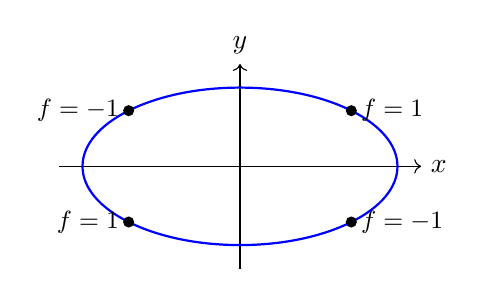
\begin{tikzpicture}[scale=1.0]
  \draw[->](-2.3,0)--(2.3,0)node[right]{$x$};
  \draw[->](0,-1.3)--(0,1.3)node[above]{$y$};
  \draw[blue,thick](0,0) ellipse (2 and 1);
  \fill( 1.414, 0.707) circle(2pt) node[right]{\small$f=1$};
  \fill(-1.414,-0.707) circle(2pt) node[left]{\small$f=1$};
  \fill( 1.414,-0.707) circle(2pt) node[right]{\small$f=-1$};
  \fill(-1.414, 0.707) circle(2pt) node[left]{\small$f=-1$};
\end{tikzpicture}
\end{center}
\end{solution}

\paragraph{Problem.} \textit{Find the point on the plane $x-y+z=4$ closest to $(1,2,3)$.}

\begin{solution}
Minimize the squared distance $d^2=(x-1)^2+(y-2)^2+(z-3)^2$ subject to $g=x-y+z-4=0$. At the closest point the level spheres of $d^2$ touch the plane, so $\nabla(d^2)$ is along the normal,
\[
  2(x-1)=\lambda,\quad 2(y-2)=-\lambda,\quad 2(z-3)=\lambda.
\]
Then $x=1+\tfrac\lambda2,\ y=2-\tfrac\lambda2,\ z=3+\tfrac\lambda2$, and the constraint gives $\lambda=\tfrac43$. The foot is $\bigl(\tfrac53,\tfrac43,\tfrac{11}{3}\bigr)$ at distance $\dfrac{2\sqrt3}{3}$. The shortest path to a plane runs along its normal, exactly what $\nabla(d^2)\parallel\nabla g$ says.
\end{solution}

\end{document}
